\documentclass{article}

% plain.bst is a numeric style, so natbib must be loaded in numeric mode; the
% template documents this hook.
\PassOptionsToPackage{numbers,compress}{natbib}

% ML4PS 2026 workshop, double-blind reviewing.
\usepackage[dblblindworkshop]{neurips_2026}
\workshoptitle{Machine Learning and the Physical Sciences}

% The submission branch of neurips_2026.sty builds the first-page footer from
% \@noticestring.  We redefine only that macro -- the mechanism the style file
% itself provides.  No style-file edits, no layout changes.
\makeatletter
\renewcommand{\@noticestring}{%
  Submitted to the 9th Workshop on Machine Learning and the Physical Sciences (ML4PS 2026). Do not distribute.%
}
\makeatother

\usepackage[utf8]{inputenc}
\usepackage[T1]{fontenc}
\usepackage{hyperref}
\usepackage{url}
\usepackage{booktabs}
\usepackage{amsfonts}
\usepackage{amsmath}
\usepackage{microtype}
\usepackage{graphicx}
\usepackage{wrapfig}

\newcommand{\qcli}{I_{\mathrm{QCLI}}}
\newcommand{\cci}{I_{\mathrm{CCI}}}
% Figures are supplied as vector PDFs; the extension is left off so that a PDF
% supersedes a PNG of the same basename automatically.
\newcommand{\figboxw}[3]{%
  \IfFileExists{#1.pdf}{\includegraphics[width=#3\textwidth]{#1}}{%
    \IfFileExists{#1.png}{\includegraphics[width=#3\textwidth]{#1}}{%
      \fbox{\parbox[c][#2][c]{0.95#3\textwidth}{\centering figure pending: \texttt{#1}}}}}}
\newcommand{\figbox}[2]{\figboxw{#1}{#2}{1.0}}

\title{IQP Generative Models for Strong Gravitational Lensing Images}

% Double-blind submission: the dblblindworkshop option suppresses the author block.
\author{}

\begin{document}

\maketitle

\begin{abstract}
Instantaneous-quantum-polynomial (IQP) circuits are believed to be hard to sample
classically~\cite{bremner_2011_classical,bremner_2016_average}, while the expectation values a
maximum-mean-discrepancy (MMD) loss needs stay computable, so an IQP Born machine can be trained
classically and deployed on quantum hardware~\cite{recio_2025_train}. A recent
correlation--complexity map, two indices computed from a dataset's Walsh order spectrum and its
multi-information, predicts which datasets suit such models, and on it DeepLense
strong-lensing images are the most IQP-compatible dataset we measured ($\qcli = 0.47$,
$\cci = 0.87$), above the turbulence data of the paper that introduced it. Given \emph{learned} latent directions,
$\theta = \theta^{0} + \Phi^{\!\top} z$, a 10-qubit IQP Born machine trained on lens crops beats an
RBM and a DCGAN on the paper's PDF--JS and on flux-aligned Conv2D-MMD$^2$ at $N = 11$ and
$N = 100$ training images with $2$--$39\times$ fewer parameters, a different arm winning each
metric, and reconstructs unseen images at correlation $0.97$. Three caveats
bound it. The reference paper's own fixed latent protocol yields only noise on images, a
structure-matched permutation null still scores $\qcli = 0.42$, and the DCGAN still leads on raw
Conv2D-MMD$^2$ at $N = 100$. Everything is exact classical simulation at a single seed and $n = 10$
qubits, so we claim no quantum advantage.
\end{abstract}

\section{Introduction}
\label{sec:intro}

IQP circuits are commuting-gate circuits whose output distribution is the squared Walsh--Hadamard
transform of a phase function. Exact classical sampling from them would collapse the polynomial
hierarchy~\cite{bremner_2011_classical}, and the hardness is conjectured to survive approximate
sampling in the average case~\cite{bremner_2016_average,codsi_2025_classically}, though sufficient
noise restores classical simulability~\cite{rajakumar_2024_polynomial}. The same commuting structure
keeps an MMD loss's expectation values computable, so such a model can be \emph{trained classically
and deployed on quantum hardware}~\cite{recio_2025_train,recio_2025_iqpopt}.

Whether real data sits where that is useful is an empirical question, and a recent
proposal~\cite{liu_2026_correlation} approaches it with two ingredients. (i) A
\emph{correlation--complexity map} placing a dataset on two coordinates, the quantum
correlation-likeness indicator $\qcli$, how much of its Walsh order spectrum sits at high order as an
IQP output would, and the classical correlation-complexity indicator $\cci$, how much of its total
correlation the best pairwise tree misses~\cite{watanabe_1960_information,schneidman_2003_network};
the high-$\qcli$, high-$\cci$ corner is argued to be where IQP circuits do well. (ii) A
latent-adaptation protocol (Algorithm~1 of the reference paper, which trains a shared phase core on
one anchor sample, then adapts a fixed block of $50$ Walsh-basis phases taken in Hamming order
sample by sample, and interpolates that block to reach unseen samples). Both were
demonstrated on one dataset, 2D turbulence snapshots~\cite{khojasteh_2022_lagrangian} at $n=18$
qubits.

We take both to simulated dark-matter strong-lensing images from
DeepLense~\cite{alexander_2020_deep,alexander_2021_decoding} and report three results. (1) Lens
crops land at the most IQP-compatible position of any dataset we measured. (2) A 10-qubit IQP Born
machine trained on those crops beats the paper's own RBM and DCGAN baselines on PDF--JS and on
flux-aligned Conv2D-MMD$^2$, a different arm winning each metric, with far fewer parameters.
(3) It does so only once the fixed Walsh latent block of the reference protocol is made
\emph{learnable}. Appendices~\ref{app:turb}--\ref{app:fig4} take the same tests back to the paper's
own data, where its turbulence result does not reproduce under our pre-registered convention and two
internal claims come out mixed.

\section{Setup}
\label{sec:setup}

\paragraph{Data and encoding.}
We use the DeepLense \texttt{Model~II} simulation set (80{,}194 train / 8{,}910 validation images,
$64\times64$, three substructure classes pooled, with per-class results in
App.~\ref{app:classes})~\cite{alexander_2020_deep,alexander_2023_domain,ml4sci_deeplense}. Each image is
centroid-aligned by an integer shift (offset $3.4 \pm 1.6$\,px) and cropped to the central
$32\times32$ window, keeping $99.4\%$ of the light, and the crop becomes a probability mass function
(pmf) $p(k_x,k_y)$ over $1{,}024$ cells on $n=10$ qubits (App.~\ref{app:pipe}). All $2^{10}$
generators $Z_s$ are used, so $\theta \in \mathbb{R}^{1024}$ and $q_\theta$ follows from two
length-$1024$ fast Walsh--Hadamard transforms.

\paragraph{Latent parameterisations.}
We compare the reference protocol against (i) its fixed $50$-phase block trained \emph{jointly}
across images and (ii) our
\emph{learned-direction} model (a trainable matrix $\Phi$ whose $M$ rows are directions in phase
space, so that each image becomes a point $z_i$ in $M$ dimensions), written
\begin{equation}
\theta_i \;=\; \theta^{0} + \Phi^{\!\top} z_i,
\qquad \theta^{0}\in\mathbb{R}^{1024},\quad
\Phi\in\mathbb{R}^{M\times 1024},\quad z_i \in \mathbb{R}^{M},
\label{eq:affine}
\end{equation}
with $M \in \{2,4,8\}$, each row of $\Phi$ $L^2$-normalised to $\sqrt{1024}$, and
$\theta^0,\Phi,\{z_i\}$ trained jointly under an $L^2$ penalty on $z$ of $10^{-3}$, raised to $0.3$
for the $M{=}8$ arm. The three objectives are the paper kernel (the reference paper's
multi-bandwidth Gaussian MMD kernel), the flat MMD (uniform weight on every Walsh coefficient, which
makes it estimable from hardware shots) and exact KL (a simulation-only diagnostic, reported in
App.~\ref{app:arms}). For unconditional generation $z$
is drawn from a fitted Gaussian or resampled from the trained $z_i$ with jitter.

\paragraph{Baselines and metrics.}
We compare only against the two baselines the reference paper uses, a restricted
Boltzmann machine (RBM; 10 visible and 1{,}000 hidden units, persistent contrastive divergence
with one Gibbs step~\cite{hinton_2002_training,tieleman_2008_training}) and a deep convolutional
generative adversarial network (DCGAN)~\cite{radford_2015_unsupervised}, both trained on the same
data and both sized in Table~\ref{tab:main}. Metrics are
the paper's two, the probability-density Jensen--Shannon divergence between intensity histograms
(PDF--JS) and Conv2D-MMD$^2$, a biased MMD estimate in the feature space of a fixed random
three-layer convolutional encoder~\cite{gretton_2012_kernel}. Every IQP arm and the RBM share the flux scalar $S$ while the
DCGAN learns its own scale, so raw Conv2D-MMD$^2$ is partly a brightness comparison and we also
report a flux-aligned variant, flagged as post-hoc. Every arm generates 200 images scored against the
same 200 held-out images at the reference training-set sizes $N \in \{11,100\}$, with a single seed
(seed 0) throughout.

\paragraph{Departures from the reference setup.}
Six choices differ from the reference paper, and each follows from the data rather than from the
model. Its snapshots carry a time index and its task is to interpolate to unseen times, whereas lens
images are static and fall into three substructure classes, so we generate unconditionally from the
latent prior and report the classes separately in App.~\ref{app:classes}. It encodes a sample as
18-bit $(x,y,\mathrm{intensity})$ tuples on $18$ qubits with the generators truncated by subset size
to about $31$k phases, whereas we encode the whole crop as one pmf on $10$ qubits and keep every
generator, because that crop already holds nearly all the light while a raw intensity axis carries
barely more than one bit, so a tuple encoding would spend qubits on
intensity when the spatial structure is what has to be learned. It fits a core on one anchor and then adapts a fixed
block of $50$ Walsh phases one sample at a time, whereas we learn the directions $\Phi$ and train the
$N$ images jointly, since fixed Walsh directions cross-fade pixels instead of moving a ring
(Sec.~\ref{sec:whyfail}). It estimates its MMD
from $500$ model samples per step, whereas at $n=10$ we evaluate it in closed form. We keep its
metrics and its baselines, the RBM reading the same 10-bit code and the DCGAN the same $32\times32$
crops, add a held-out projection correlation, and paste each generated crop back into $64\times64$ at a fixed flux $S = 124.92$ and a sampled
offset before scoring.

\begin{figure}[t]
\centering
\figbox{figures/fig1_compact}{2.3in}
\caption{\textbf{(a)} Correlation--complexity map, with datasets filled, i.i.d.-uniform nulls at the
same $(n,K)$ open and labelled null, and permutation nulls as crosses labelled perm.\ null (ours, not
in the reference paper). The legend also shortens lens 18b for the 18-bit per-image encoding, lens
18b pool for its pooled variant, lens 10b for the 10-bit crop pmf, turb.\ D2 and D2 pooled for the
reference paper's turbulence data, and Blobs for BinaryBlobs.
\textbf{(b)} First three unconditional samples per model, $N{=}100$, no selection, shared $0$--$1$
colour scale (at most 13 pixels per row are clipped), where IQP ref.\ is the reference protocol and
IQP $M{=}4$ our flat-MMD arm.}
\label{fig:map}
\end{figure}

\section{Results}
\label{sec:results}

\subsection{Lens images are the most IQP-compatible dataset on the map}
\label{sec:map}

Encoded as the reference paper encodes turbulence, at $K = 4{,}096$ sampled tuples per image, the
lens images of Fig.~\ref{fig:map}(a) score
$\qcli = 0.4715$ and $\cci = 0.8677$, higher in $\qcli$ than the paper's own
turbulence data at the same $K$ ($0.023$), binarised MNIST ($0.014$) or BinaryBlobs ($0.032$, both at
$K = 10^{4}$), and inside the map's IQP-compatible corner.

A permutation null that keeps each image's intensity histogram and destroys all spatial structure
still scores $\qcli = 0.4154$ and \emph{raises} $\cci$ to $0.8782$, leaving only $+0.056$ in $\qcli$
from lens structure, and the paper's own turbulence data behaves the same way, so at this encoding
the map largely tracks the intensity histogram. The 10-bit crop pmf we train on does separate from its
permutation null in both coordinates ($\qcli$ $0.473$ against $0.178$, $\cci$ $0.431$ against
$0.963$), and we therefore read a favourable map position as necessary rather than sufficient.

\subsection{Why the reference protocol needs learned directions}
\label{sec:whyfail}

Run sequentially on our low-variance latent block, Algorithm~1 produces noise
(Fig.~\ref{fig:map}(b), second row; the Hamming-ordered variant is in App.~\ref{app:arms}).
Representability is not the cause, since the full 1{,}024-phase circuit fits a \emph{single} aligned
crop to correlation $0.99997$ under the flat MMD and $0.9962$ under the paper kernel. The
protocol is. With the core frozen on one anchor, the 50 fixed latent coordinates reconstruct every
other training image at correlation $0.47$, because fixed Walsh directions act as an XOR-shift
interference pattern that cross-fades pixels instead of moving lens structure, which suits a drifting
time series and not an i.i.d.\ image set.

\subsection{Learned latent directions generalise}
\label{sec:affine}

Equation~\eqref{eq:affine} repairs this. To test generalisation we freeze $\theta^{0}$ and $\Phi$
and optimise only $z$ on 200 \emph{held-out} images. At $N{=}100$ the best arm, flat MMD at
$M{=}4$, reaches mean correlation $0.968$ (minimum $0.851$) against a nearest-training-image
reference of $0.970$, while the paper kernel reaches only $0.74$--$0.79$. The gain comes from
learning the directions and not from the extra
parameters, since in the controlled $N{=}20$ sweep of Fig.~\ref{fig:gen}(a) a trained $\Phi$ reaches
$0.911$ against $0.672$ for a random $\Phi$ of the same size. Useful $M$ stays small, collapsing to $0.095$ by $M{=}8$ once the required $\|z\|$ exceeds the model's
coherence radius ($\approx 0.03$--$0.05$).

\begin{table}[t]
\centering
\caption{Paper-style comparison on lens crops, IQP against the two baselines the reference paper
uses. Lower is better and \textbf{bold} marks the best entry in a column. Learned-direction parameter
counts are $N{=}11\,/\,N{=}100$, and MMD$^2_{\mathrm{al}}$ is the flux-aligned variant
(post-hoc). The last row is an empirical floor from scoring one held-out half against the other, not
a model. Single seed.}
\label{tab:main}
\scriptsize
\setlength{\tabcolsep}{4.5pt}
\begin{tabular}{lrccc@{\hskip 10pt}ccc}
\toprule
& & \multicolumn{3}{c}{$N = 11$} & \multicolumn{3}{c}{$N = 100$} \\
\cmidrule(lr){3-5}\cmidrule(lr){6-8}
Model & Params & PDF--JS & MMD$^2$ & MMD$^2_{\mathrm{al}}$ & PDF--JS & MMD$^2$ & MMD$^2_{\mathrm{al}}$ \\
\midrule
IQP, paper protocol (Alg.~1)      & 1{,}024          & 0.00609 & 0.2031 & 0.1837 & 0.00697 & 0.2140 & 0.2233 \\
IQP, fixed basis, joint           & 1{,}024          & 0.00133 & 0.1416 & 0.1141 & 0.00099 & 0.1041 & 0.0617 \\
IQP, learned dir.\ $M{=}4$ (flat MMD) & 5{,}164 / 5{,}520 & 0.00196 & 0.1134 & \textbf{0.0279} & 0.00239 & 0.0861 & \textbf{0.0275} \\
IQP, learned dir.\ $M{=}4$ (paper kernel) & 5{,}164 / 5{,}520 & \textbf{0.00095} & 0.1168 & 0.0679 & \textbf{0.00092} & 0.1189 & 0.0876 \\
RBM~\cite{tieleman_2008_training}  & 11{,}010        & 0.00632 & \textbf{0.0741} & 0.1240 & 0.00195 & 0.0752 & 0.1144 \\
DCGAN~\cite{radford_2015_unsupervised} & 199{,}837   & 0.00183 & 0.2165 & 0.1241 & 0.00763 & \textbf{0.0371} & 0.0694 \\
\midrule
\textit{Held-out split-half (floor)} & n/a & \textit{0.00003} & \textit{0.0040} & \textit{0.0069} & \textit{0.00003} & \textit{0.0040} & \textit{0.0069} \\
\bottomrule
\end{tabular}
\end{table}

\subsection{Paper-style comparison and data scaling}
\label{sec:table}

In Table~\ref{tab:main} the $M{=}4$ paper-kernel arm wins PDF--JS at both training-set sizes
($0.00095$ and $0.00092$) and the $M{=}4$ flat-MMD arm wins the flux-aligned Conv2D-MMD$^2$ at both
($0.0279$ and $0.0275$), with $2\times$ fewer parameters than the RBM and $39\times$ fewer than the
DCGAN, though no single arm wins both metrics. Two of the four IQP arms fall behind the DCGAN on
PDF--JS at $N{=}11$ and two fall behind the RBM at $N{=}100$, and on raw Conv2D-MMD$^2$ the IQP
arms \emph{lose} to the RBM at $N{=}11$ ($0.0741$ against $0.1134$) and to
the DCGAN at $N{=}100$ ($0.0371$ against $0.0861$), an ordering that reverses once flux is aligned.
The paper's data-scaling claim holds only in part, since our DCGAN is \emph{better} at $N{=}11$ than
at $N{=}100$ on PDF--JS, the opposite of the low-data GAN collapse the paper reports
(Fig.~\ref{fig:scaling}, App.~\ref{app:arms}). Trained on each substructure class on its own, the same arm reaches the same
level (App.~\ref{app:classes}).

\begin{figure}[t]
\centering
\figbox{figures/fig2_compact}{2.0in}
\caption{Panels (a) and (b) are different experiments. \textbf{(a)} Controlled latent-width sweep
($N{=}20$ mechanism test), held-out projection correlation against the number of learned directions
$M$, with its own reference levels ($0.934$ nearest training image, $0.744$ mean training image,
$0.672$ random directions); the $M{=}8$ and $16$ points are the best over a learning-rate
sweep, i.e.\ favourable to the model. \textbf{(b)} Round-3b arms at $N{=}100$, held-out crops on top, then
$M{=}4$ under the flat MMD, $M{=}4$ under the paper kernel, and the collapsed $M{=}8$ arm, which was
trained with KL and a $z$-penalty.}
\label{fig:gen}
\end{figure}

\section{Discussion and limitations}
\label{sec:disc}

The map places lens images where IQP models should do well and the runs bear that out on both
metrics, one arm for each, but only with learned latent directions. Nothing here is evidence of
quantum advantage, because every circuit is
simulated exactly at $n=10$ qubits and the hardness results describe the model class at scale
rather than our instances. All numbers are single seed, and the DCGAN's $3\times$ swing in
Fig.~\ref{fig:scaling} sets the scale of the effects we discuss. The imposed flux scalar leaves raw
Conv2D-MMD$^2$ partly a brightness metric and the aligned variant post-hoc, and zero-learning and
PCA controls match or exceed the IQP arms on some physical-quantity metrics.

\bibliographystyle{plain}
\bibliography{refs}

\newpage
\appendix

\section{Pipeline}
\label{app:pipe}

Figure~\ref{fig:pipe} summarises the encoding, the latent parameterisation and the evaluation.

\begin{figure}[h]
\centering
\figboxw{figures/fig_pipeline_v2}{3.6in}{0.92}
\caption{Pipeline. \textbf{(a)} A held-out $64\times64$ image, white cross at its intensity centroid
and dashed box the $32\times32$ crop window. \textbf{(b)} The aligned crop read as a pmf over
$1{,}024$ cells, where the example pixel $(k_x,k_y) = (12,20)$ carries code $404 = 0110010100_2$ and
bit $j$ addresses qubit $j$. \textbf{(c)} The first two learned latent coordinates of the $100$
training images at $M = 4$. \textbf{(d)} The IQP circuit, an H layer, one diagonal phase
$\exp(i\sum_s \theta_s Z_s)$ over all $1{,}024$ subsets $s$, a second H layer and measurement.
\textbf{(e)} Exact simulation through $q_\theta = |\mathcal{W}e^{i\theta}|^{2}/2^{n}$, trained jointly
over the $N$ images by MMD (flat or reference kernel) or by KL, the dashed arrow updating
$\theta^{0}$, $\Phi$ and $z$. \textbf{(f)} A trained $q(x,y)$ scaled by $S$ and pasted at a sampled
offset. \textbf{(g)} The intensity PDF of real against IQP samples (PDF--JS $0.0024$), Conv2D-MMD$^2$
at $N{=}100$ (IQP $0.086$, RBM $0.075$, DCGAN $0.037$), and projection correlations over $200$
held-out images (mean $0.968$). The bottom row contrasts a reference-protocol sample with an $M{=}4$
sample from this work.}
\label{fig:pipe}
\end{figure}

\section{Replication of the reference paper's turbulence experiment}
\label{app:turb}

We attempted a direct replication on the reference paper's own dataset (2D cylinder-wake turbulence
D2~\cite{khojasteh_2022_lagrangian}, $n=18$ qubits, 11 anchor snapshots). Under
our pre-registered evaluation convention the result is \textbf{not reproduced},
since in the 11-snapshot regime the RBM and a 1.2M-parameter DCGAN beat our IQP on \emph{both} of the
paper's metrics. Two findings qualify this. Under a last-write-wins aggregation convention, never
specified in the paper, our IQP's PDF--JS values do land close to the published ones ($0.0322$ and
$0.0476$ against $0.0238$ and $0.0221$), but the RBM still wins. Conv2D-MMD$^2$ is also saturated
there, since ground truth shuffled in
pixel space already scores $0.704$, below every model in the paper's Table~2 ($0.90$--$1.47$), and
the unseen-time synthesis task is solvable by linear interpolation (correlation $0.9998$). Our
anchor-fit ceiling (correlation $0.69$ sampled, $0.77$ exact) traces to a frozen
$\theta_{\mathrm{lat}}$ in stage~1 ($\approx -0.08$), a $5\times10^{4}$-sample pmf ($\approx -0.04$)
and a $0.88$--$0.89$ model-family ceiling, not to our implementation.

\section{Support mismatch (reference paper Fig.~3)}
\label{app:fig3}

\begin{figure}[h]
\centering
\begin{minipage}[t]{0.38\textwidth}\centering
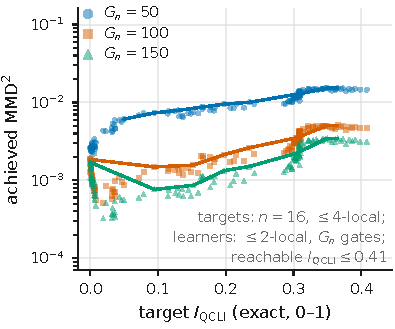
\includegraphics[width=\linewidth]{figures/figA_fig3}
\end{minipage}\hfill
\begin{minipage}[t]{0.38\textwidth}\centering
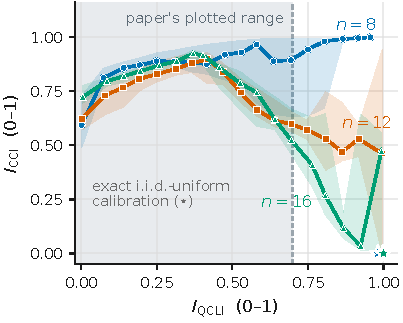
\includegraphics[width=\linewidth]{figures/figA_fig4}
\end{minipage}
\caption{\textbf{(a)} Support-mismatch study at $n=16$, with $140$ target circuits ($\leq 4$-local)
spanning exact $\qcli \in [0, 0.408]$ fitted by $\leq 2$-local learners of $50$, $100$ and $150$
gates (exact MMD, Adam, $5{,}000$ steps). More gates lower the whole envelope (claim (b),
reproduced), while within the reachable range the achieved MMD$^2$ \emph{rises} with target $\qcli$,
the opposite of claim (a). \textbf{(b)} Circuits optimised to maximise $\qcli$ only, $n = 8, 12, 16$,
3 seeds and 2 gain settings per $n$, $3{,}333$ steps each and about $20{,}000$ logged points per $n$.
$\cci$ never enters the objective.}
\label{fig:appcd}
\end{figure}

The reference paper's Fig.~3 claims (a) that the upper envelope of achievable MMD falls as the
target's $\qcli$ rises, because the support-induced floor shrinks, and (b) that the envelope drops
overall as the learner gets more gates (Fig.~\ref{fig:appcd}(a)). Claim (b) reproduces, as the median
achieved MMD$^2$ falls $9.57\times10^{-3} \to 2.15\times10^{-3} \to 1.45\times10^{-3}$ across the three
learners. Claim (a) runs the other way inside the range we can reach, since the achieved MMD$^2$
\emph{rises} as the target's exact $\qcli$ goes from $0$ to $0.41$ (Spearman
$\rho = +0.98/+0.90/+0.81$), a trend that also holds for a control trained on exact pmfs. The paper's premise still holds mechanistically ($\rho \le -0.98$ for the
Proposition~II.2 floor proxy), but here the achieved MMD is dominated by trainability rather than by
support mismatch. Our target family saturates at exact $\qcli \approx 0.41$, and at $0$--$0.064$ when
estimated from $10^{4}$ samples as the paper does, so the regime where claim (a) is asserted lies
outside what we could construct.

\section{\texorpdfstring{The $\qcli$--$\cci$ ceiling}{The QCLI-CCI ceiling}}
\label{app:fig4}

We also reproduced the experiment in which maximising $\qcli$ alone raises $\cci$ as a by-product
(Fig.~\ref{fig:appcd}(b)). The coupling reproduces at low $\qcli$
(Spearman $\rho = +0.83/+0.76/+0.95$ for $n=8/12/16$ restricted to $\qcli \leq 0.3$) but reverses
above $\qcli \approx 0.38$ for $n = 12,16$ (global $\rho = -0.53, -0.57$). The reversal is forced by
the definitions, because the exactly uniform distribution maximises $\qcli$ ($0.982/0.998/1.000$ for
$n=8/12/16$) and has $\cci = 0$. The reference paper's figure stops below $\qcli \approx 0.7$, so a
high $\qcli$ need not indicate exploitable structure and can simply indicate proximity to uniform.

\section{Additional arms}
\label{app:arms}

\begin{wrapfigure}{r}{0.50\textwidth}
\vspace{-1.1\baselineskip}
\centering
\figboxw{figures/figA_scaling}{2.1in}{0.48}
\caption{Conv2D-MMD$^2$ against training-set size, raw as solid lines and flux-aligned as dashed
lines with open markers, over the band of the held-out split-half floor.}
\label{fig:scaling}
\vspace{-0.8\baselineskip}
\end{wrapfigure}

\paragraph{Data scaling.} At $N \in \{10,30,50,70,90,100\}$ the learned-direction IQP arm is flat for
$N \geq 30$ (raw Conv2D-MMD$^2$ $0.082$--$0.087$) and so is the RBM ($0.066$--$0.089$), while the
DCGAN leads already at $N{=}10$ ($0.044$ against $0.120$) and swings by $3\times$
non-monotonically ($0.113 \to 0.037$), as Fig.~\ref{fig:scaling} shows.

\paragraph{Exact KL.} KL needs the full simulated distribution and cannot be estimated from
hardware shots, so we keep it out of Table~\ref{tab:main} and record it here. Its $M{=}2$ arm, on
$3{,}094$ / $3{,}272$ parameters, reaches PDF--JS $0.00175$ at $N{=}11$ and $0.00302$ at $N{=}100$,
with raw Conv2D-MMD$^2$ $0.1673$ and $0.1356$ and flux-aligned $0.0559$ and $0.0866$. The collapsed
$M{=}8$ arm of Fig.~\ref{fig:gen}(b) is also a KL arm.

\paragraph{Prior draws at $M{=}2$.} All draws from the $M{=}2$ prior are rings of rms radius
$9.40 \pm 0.21$\,px against $9.21 \pm 0.15$ for real data, though under-dispersed in ellipticity
($0.048$ against $0.099$).

\paragraph{Other arms.} We ran 25 conditions, 16 IQP arms, the RBM and DCGAN baselines and seven
zero-learning or PCA controls. The arms outside Table~\ref{tab:main} (Hamming-ordered latent block,
other objectives and priors, a pseudo-time conditional arm) and the controls are scored under the
same metrics in the released tables. Trained jointly rather than sequentially, the Hamming-ordered
latent block of the reference protocol reaches PDF--JS $0.00137$ at $N{=}11$ and $0.00139$ at
$N{=}100$, so what fails in Sec.~\ref{sec:whyfail} is the sequential protocol and not the choice of
block, and we did not run the Hamming block under the sequential protocol. Every IQP arm keeps a
nearest-neighbour distance to the held-out set ($3.6$--$5.9$) far above the split-half floor ($0.95$),
so none is memorising the training set, and the $M{=}8$ arm collapses (PDF--JS $0.0103$, MMD$^2$
$0.244$ at $N{=}100$).

\section{Per-class generation}
\label{app:classes}

Every result in the main text pools the three substructure classes. To check that pooling is not
hiding a class that fails, we retrained the arm of Table~\ref{tab:main} ($M{=}4$, flat MMD, resample
prior, seed 0) separately on each class and scored each run against $200$ held-out images of that
same class, changing nothing else. At $N{=}100$ all three classes land at the pooled arm's level on
every metric of Table~\ref{tab:classes}, and at $N{=}11$ all three still train, with held-out
projection correlations near $0.9$. Each class is scored against its own held-out set, which carries
its own split-half floor, so the rows compare with their pooled counterpart rather than with each
other. The samples in Fig.~\ref{fig:classes} look alike across classes, which is what the data
implies since the three differ in only a few per cent of the pixel variance, and we claim that each
class can be generated on its own, not that the model separates them.

\begin{table}[h]
\centering
\caption{Per-class generation with the arm of Table~\ref{tab:main}, each run trained on one class
and scored against $200$ held-out images of that class, with the pooled arm at the matching $N$ for
reference and lower better in every column except the projection correlation.}
\label{tab:classes}
\scriptsize
\setlength{\tabcolsep}{6pt}
\begin{tabular}{lrcccc}
\toprule
Training set & $N$ & PDF--JS & MMD$^2$ & MMD$^2_{\mathrm{al}}$ & proj.\ corr. \\
\midrule
axion only  & 11 & 0.002197 & 0.1015 & 0.02636 & 0.9232 \\
cdm only    & 11 & 0.002174 & 0.1108 & 0.02031 & 0.9238 \\
no sub only & 11 & 0.001102 & 0.08096 & 0.02379 & 0.8998 \\
\textit{pooled} & 11 & \textit{0.001963} & \textit{0.1134} & \textit{0.02786} & \textit{0.9092} \\
\midrule
axion only  & 100 & 0.002050 & 0.09012 & 0.02346 & 0.9720 \\
cdm only    & 100 & 0.002275 & 0.09783 & 0.01848 & 0.9686 \\
no sub only & 100 & 0.002001 & 0.1034  & 0.02773 & 0.9703 \\
\textit{pooled} & 100 & \textit{0.002387} & \textit{0.08607} & \textit{0.02745} & \textit{0.9684} \\
\bottomrule
\end{tabular}
\end{table}

\begin{figure}[h]
\centering
\figboxw{figures/figB_classes}{2.1in}{0.70}
\caption{Per-class samples. Each row is one class, two held-out images followed by three generated by
the arm trained on $100$ images of that class alone, taken as the first two and the first three in
index order with no selection, on the shared $0$--$1$ colour scale.}
\label{fig:classes}
\end{figure}

\end{document}
